%DataLogging
%%swith to your GitHub not done yet.
\chapter{DataLogging}
It today's lab, we are going to measure temperature. We will use a transducer that turns temperature (energy of the air molecules around us) into a voltage. So we are still learning to use transducers. But instead of concentrating on validating a physical model for temperature, we are going to concentrate on building an independent system to measure temperature, one that doesn't have to be connected to our computer.

Often we need to have a data collection device that can operate far from our computer, but still save data for later use. For example, if you were to launch your Arduino-instrument on a high altitude balloon.

Today we all need to be able to have our Arduino collect data and save it with no computer attached. We will do this using a shield. An Arduino shield fits over the top of your Arduino, connecting to the necessary pins to do its job. The other pins are still available to use for other measurements. 

	\begin{figure}[h!] 
	\centering
	\caption{Top of a prototyping shield}
	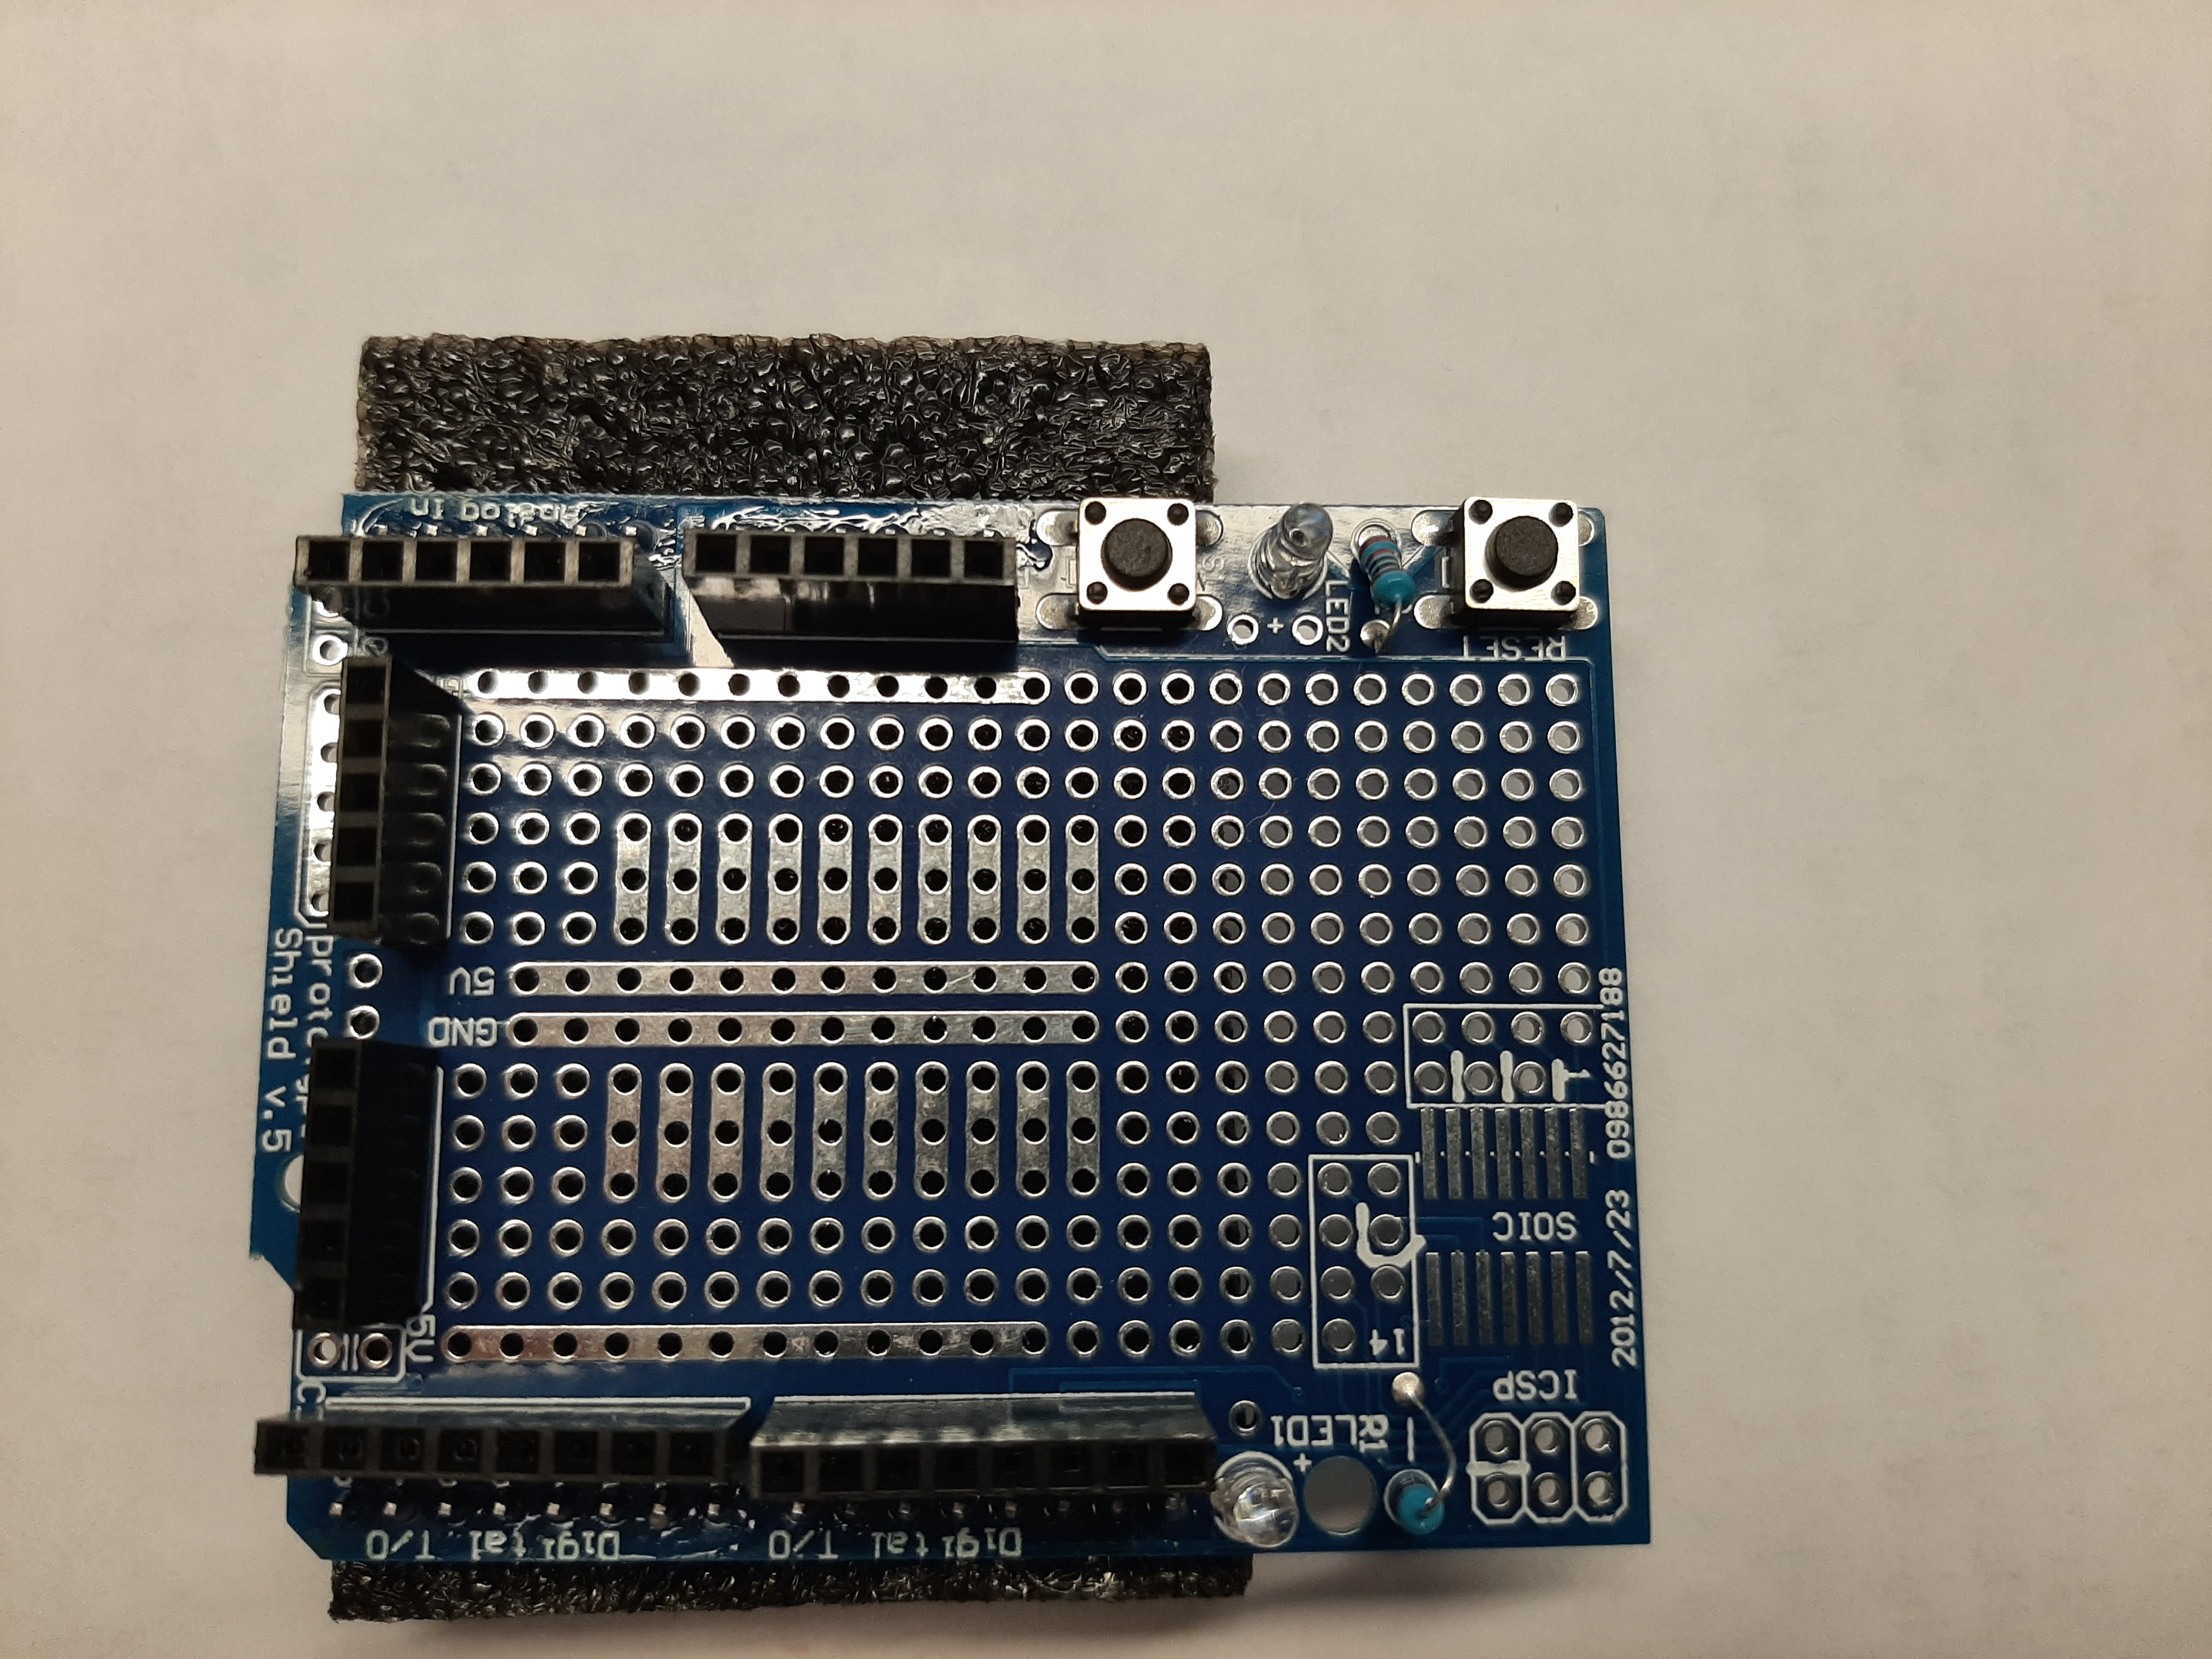
\includegraphics[width=3.614in,height=2.3981in]{20200309_133406}
\end{figure}
\section{Arduino Shields}
	Arduino shields are a simple way to add specific functionality to your Arduino. There are many different shields with many different features. Some shields have additional integrated circuit (IC) chips on them that can add additional computational power.  Others are extremely simple and are designed so you can have a more solid electrical connections with your experiment.  The previous figure and the next figure are the top and bottom of an example of a simple prototyping shield.

	\begin{figure}[h!] 
		\centering
		\caption{Bottom of a prototyping shield}
		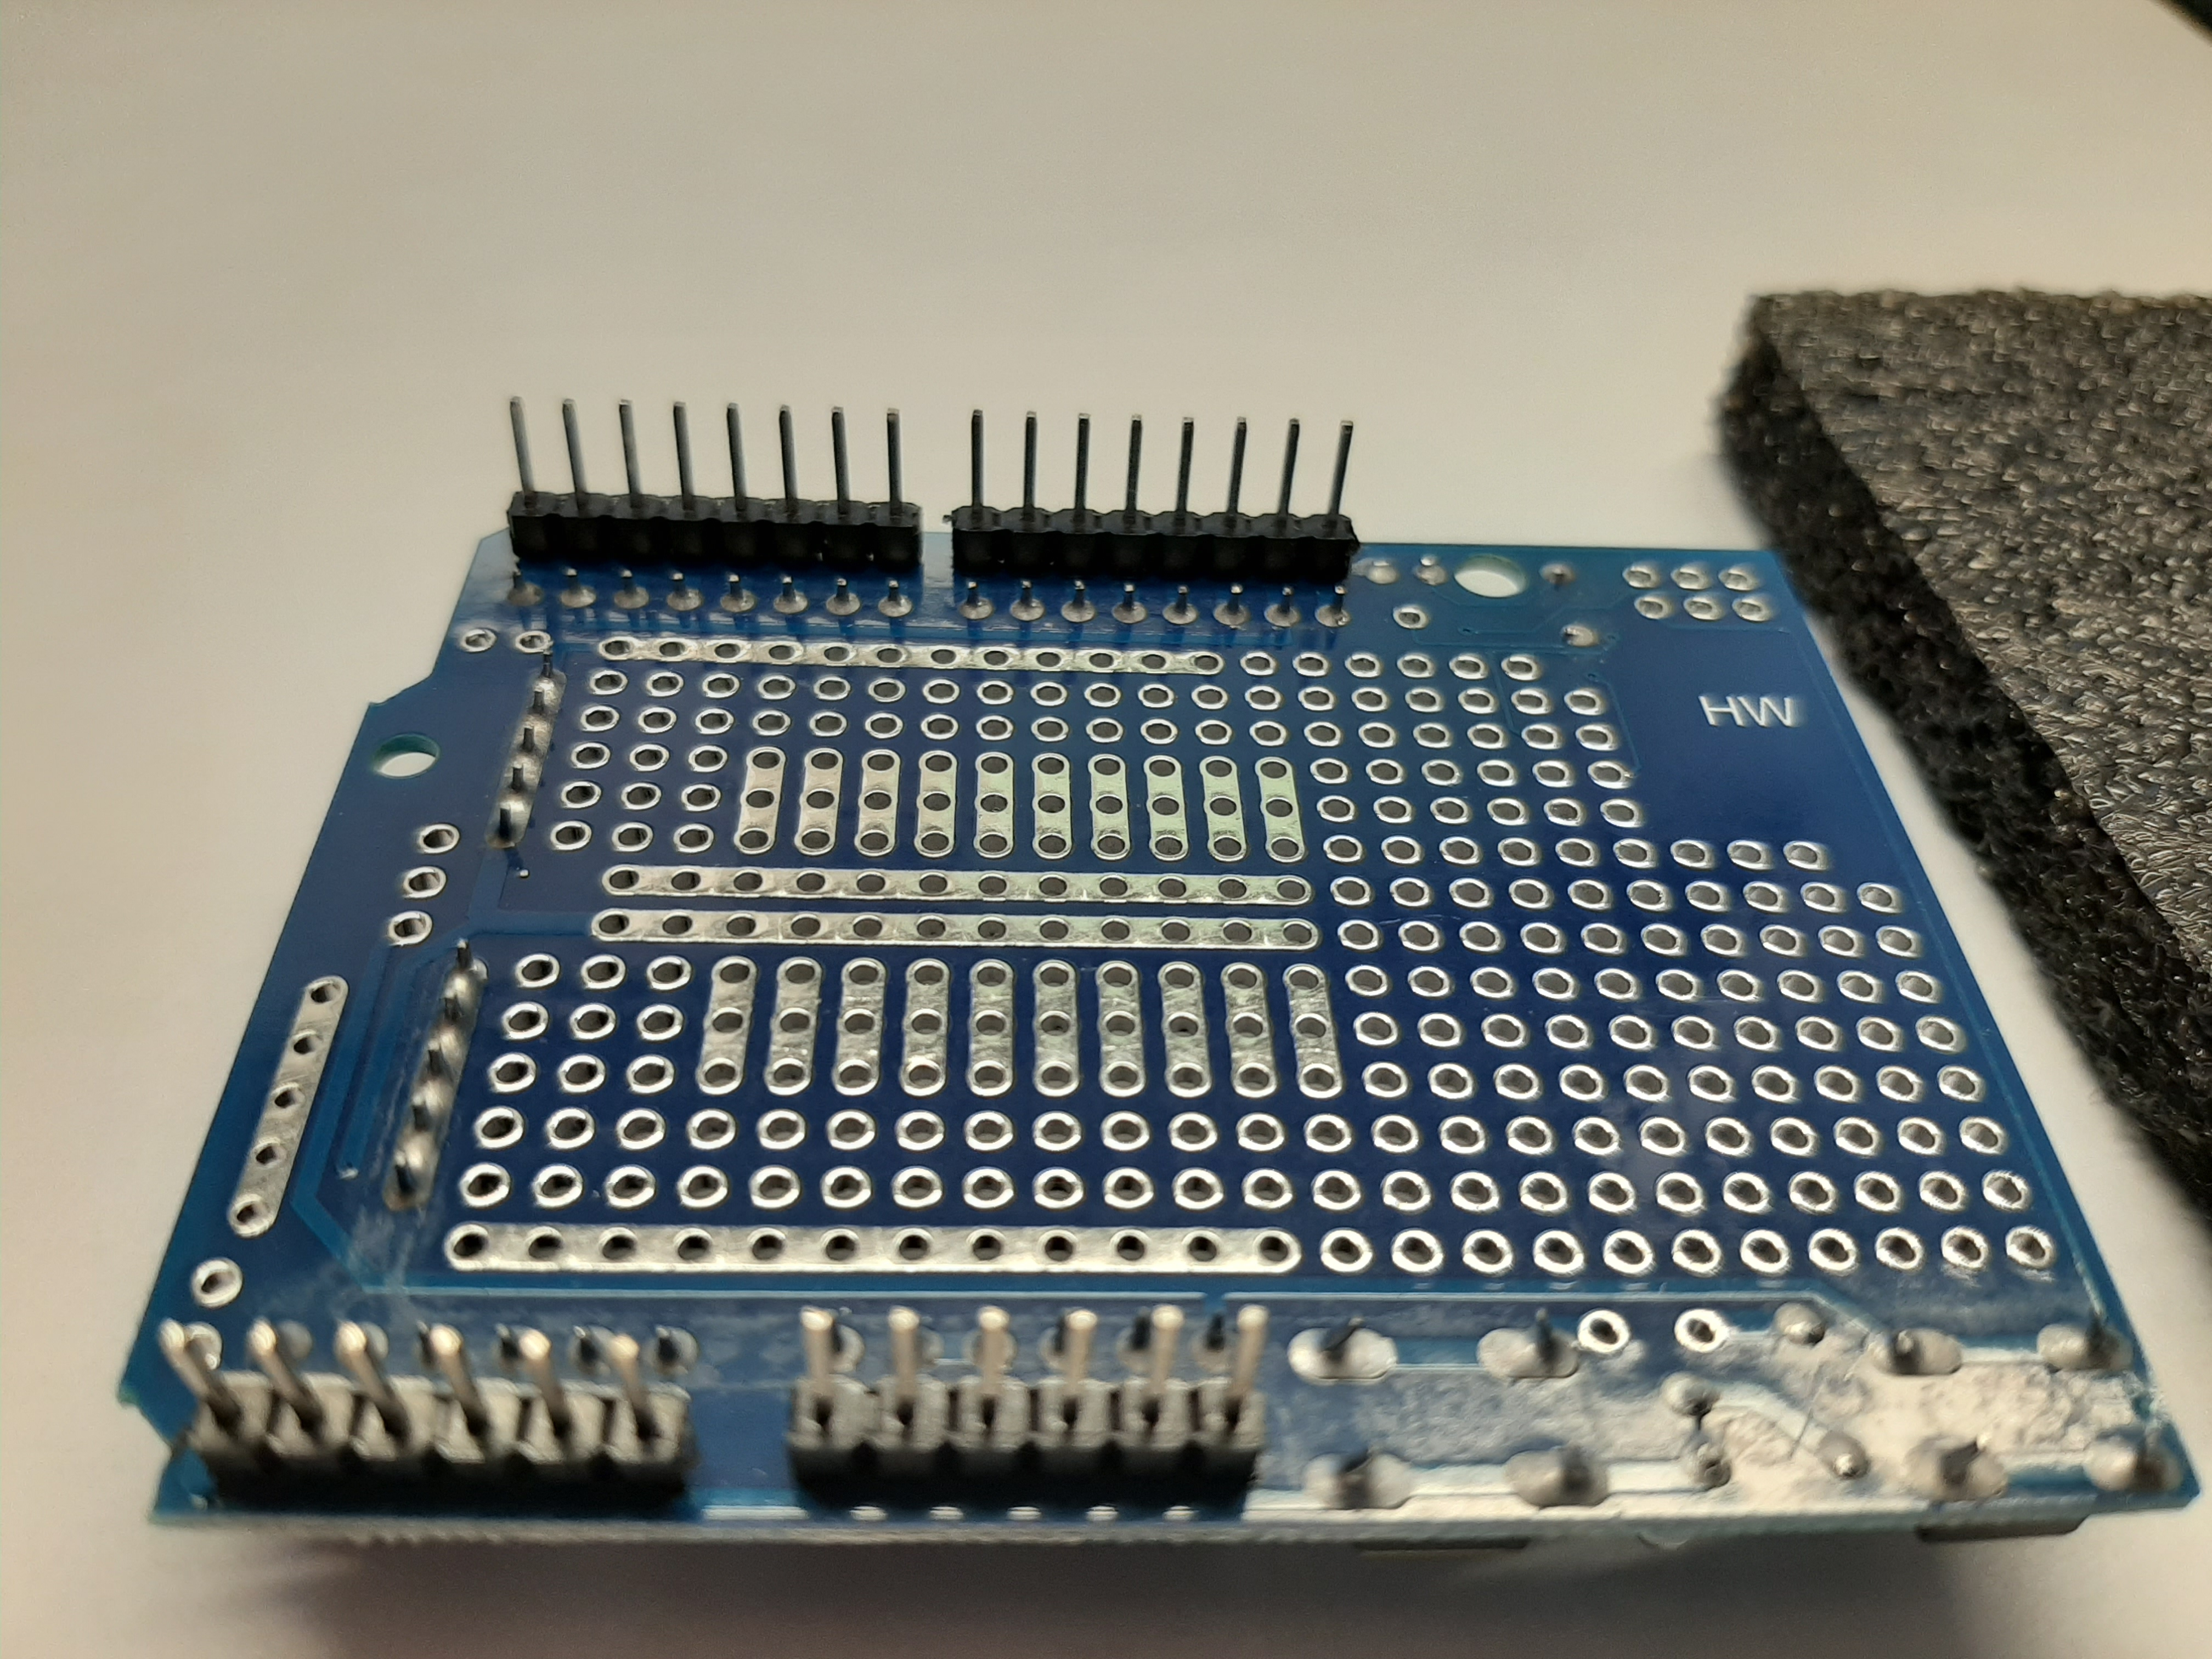
\includegraphics[width=3.614in,height=2.3981in]{20200309_133450}
	\end{figure}
	
	Notice the long wire pins on the bottom. These are designed to be plugged in directly into the Arduino. When not in use these should be pushed into the conductive foam. This will not only protect them from getting bent, but will also protect the electrical circuits on the shield from static shocks.
	
	Many shields are compatible with other shields such that they can be stacked onto each other. This will depend on what pins each shield is using and on the physical placement of both the bottom and top pins.
	
	Because shields are designed for a specific functionality the manufactures will often provide example code that utilizes those features. This code can then be modified and/or combined with other code to get your Arduino to do what ever you want. While working with shields be aware of the pins that the shield is using. So you don't interfere with its operation use other pins for your experiments.

\section{Data Logger Shield}
	Data logging is one of the most important parts of any experiment. Data for many experiments often depend on time. The data logger shield allows us to not only save the data to an SD card but we can also save the time along with it. This is because it has a built in real time clock(RTC). The data logger shield is shown in the next figure.
	
	Take a close look at the figure \ref{Data_Logger}. You will notice that the SD card slot (right next to the words ``Data logger Shield'') is close to an integrated circuit (IC). That IC (a black rectangle) controls the SD card. 
	
	There is also a battery holder. It has a battery in it, but the image also shows a piece of blue paper covering both sides of the battery. This is for shipping so that the battery isn't drained while not in use. The battery is needed for the real time clock. So that it keeps time even if there is no other power to the board. The electronics for the RTC are right next to the battery. Note the smaller IC and the silver cylinder. The cylinder holds a small quartz crystal tunning fork that keeps oscillating. These oscillations are counted by the IC and are used to keep time. 
	\begin{figure}[h!] 
		\centering
		\caption{Top of Data Logger Shield}
		\label{Data_Logger}
		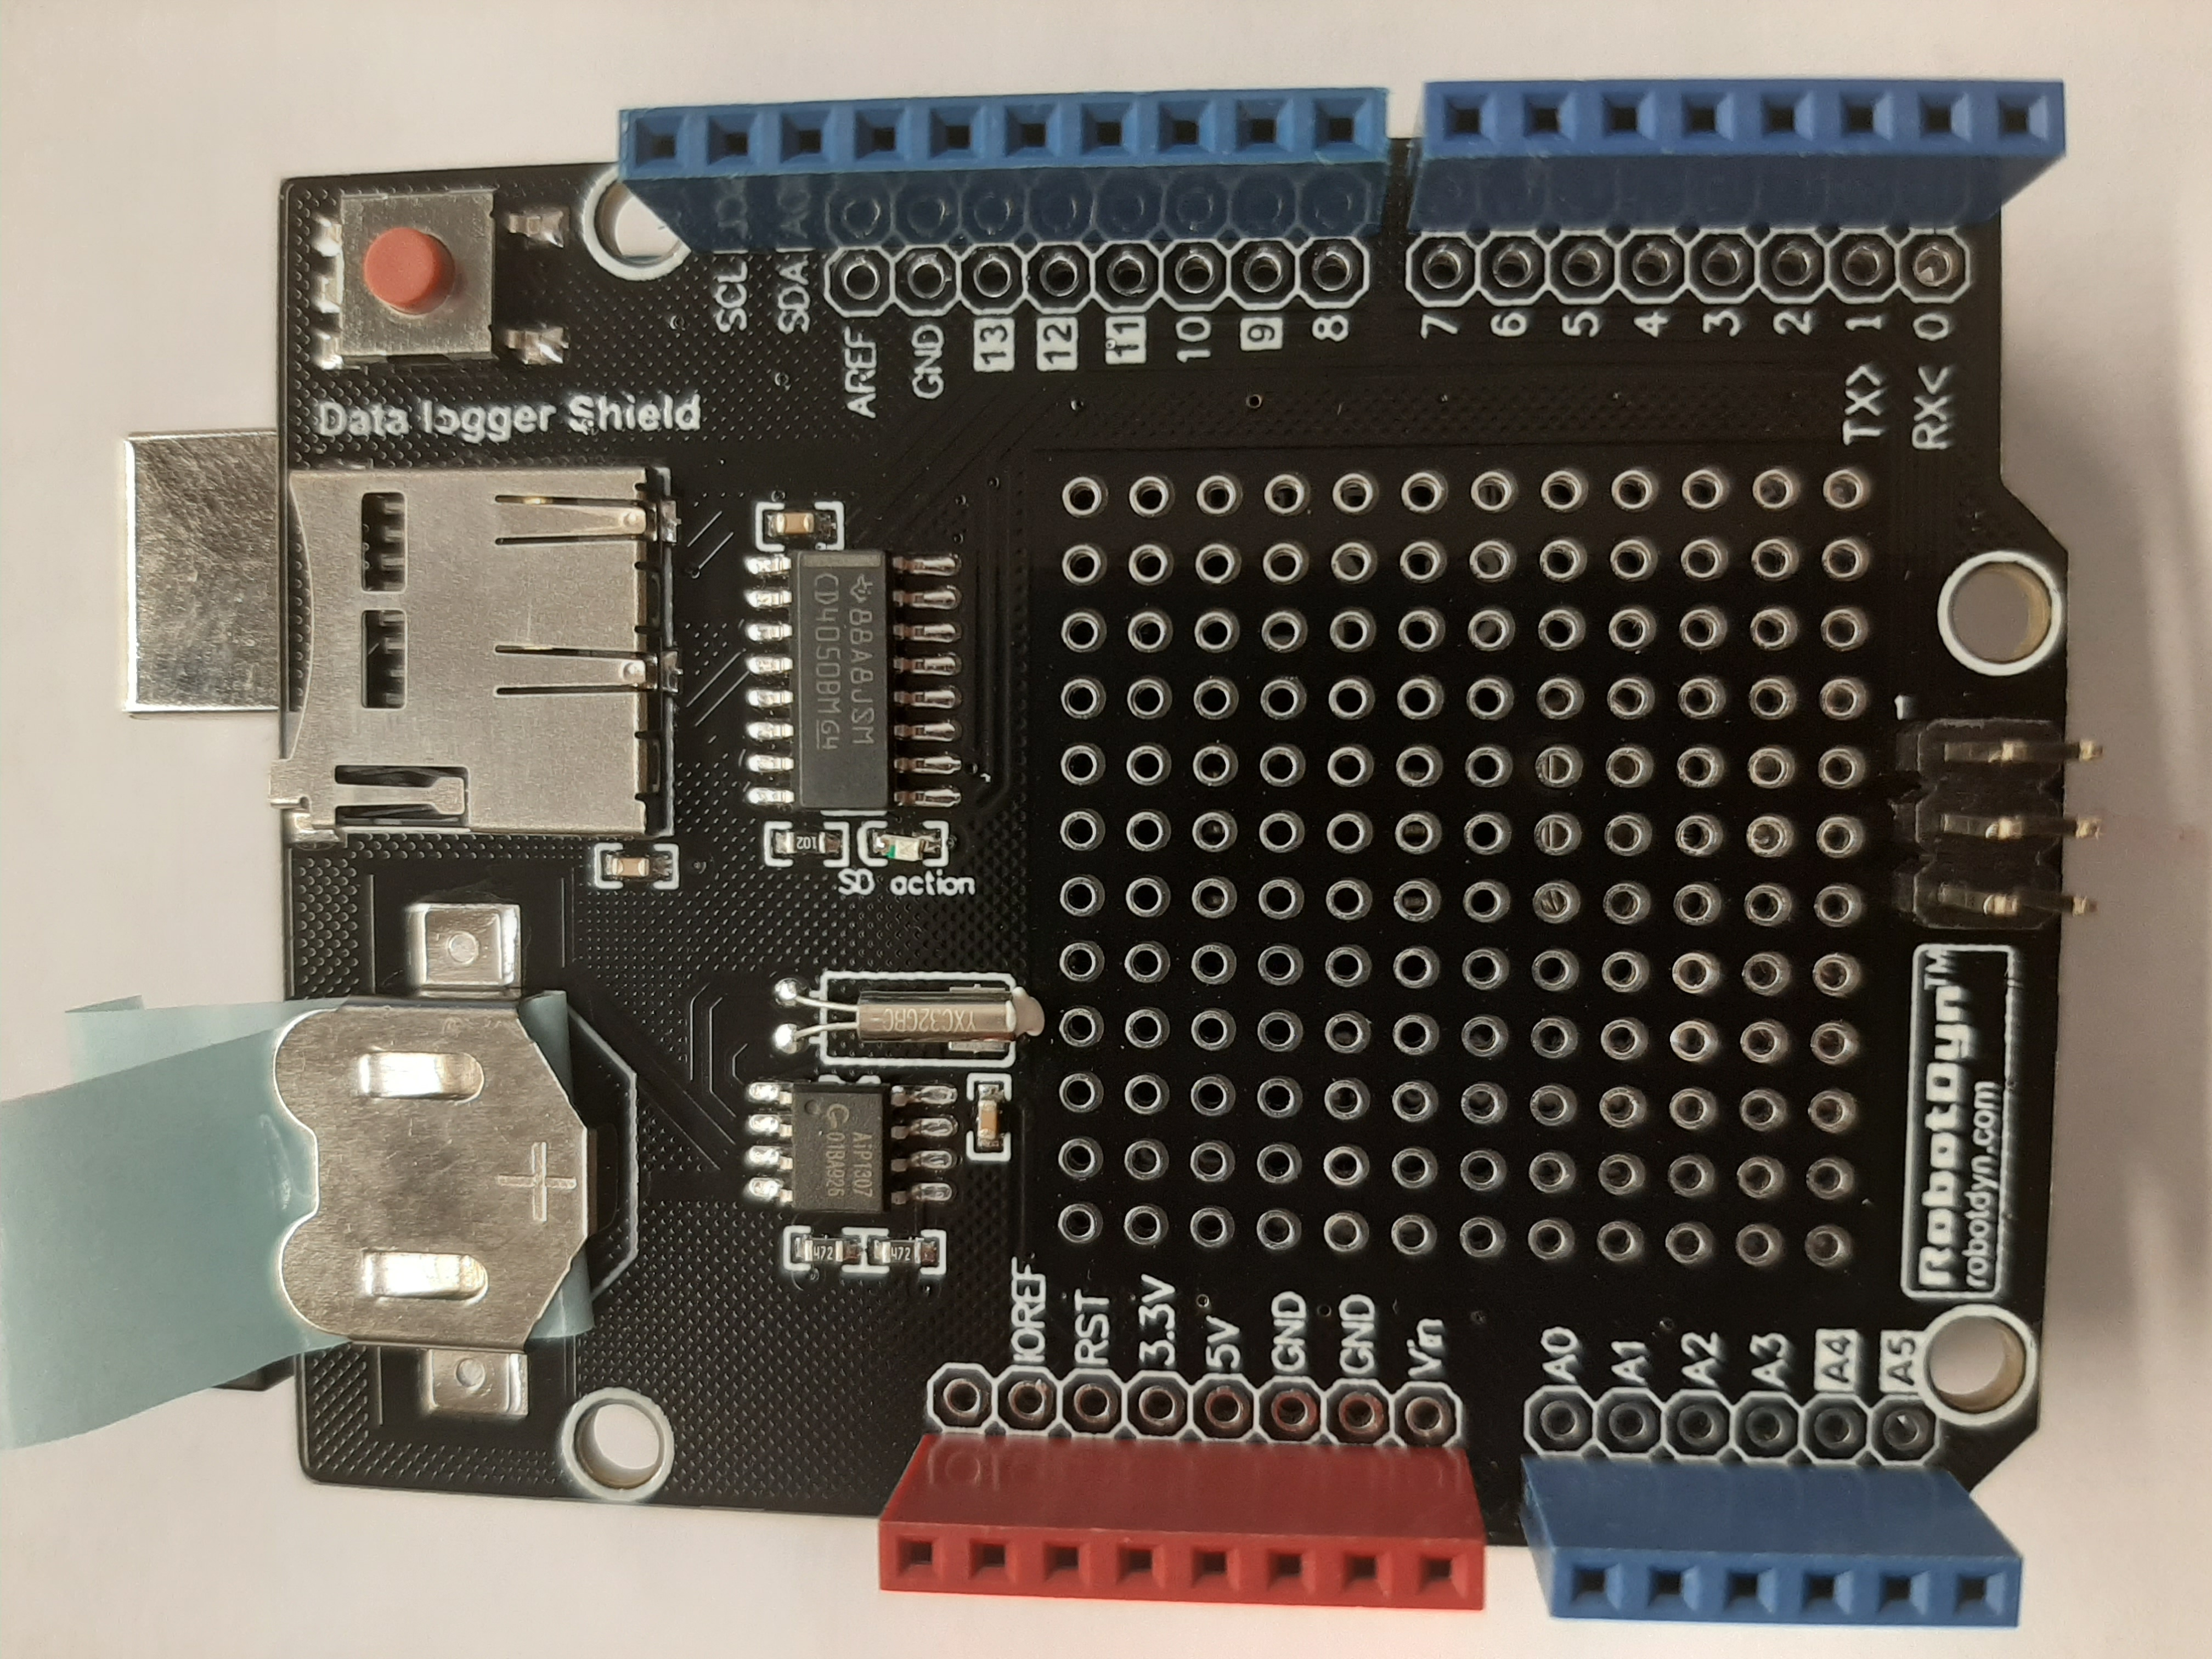
\includegraphics[width=3.614in,height=2.3981in]{20200310_110036}
	\end{figure}
	
	Just like on your Arduino the pins are all labeled. But notice that some of the pins are labeled with a white square and a back number. These pins (A4, A5, 9,11,12 and 13) are the pins that the shield uses for its functions. Make sure that your experiment doesn't use these pins. Pins A4 and A5 are used for the RTC and pins 9,11,12 and 13 are used for the SD card. The bottom of shield gives additional labels to these pins that describe their function. 



\section{Set up}
	The Data Logger shield uses a library. To get that library follow these steps in the Arduino software.
	\begin{enumerate}
		\item Under "Tools" go to ``Manage Libraries ...''
		\item Search for ``RTClib''
		\item Find the library by Adafruit and install it.
	\end{enumerate}

    The first time the software is run on the Arduino with the Data Logger shield the RTC needs to be set.  Pull out the paper that keeps the battery from contacting  and put the battery back (if the paper is still there). Then upload the code below. Check the serial monitor. If it says that the ``RTC has not been set!'' or if the date and time are incorrect then you will need to remove the comment back slashes on the line 
    \begin{lstlisting}[language=Arduino]
   		 rtc.adjust(DateTime(2014, 1, 21, 3, 0, 0));
    \end{lstlisting}
    But change the numbers to match the current date and time. Then upload the code again. This will set the clock. This only needs to be done once, as the battery will keep time from then on. So put the comment back slashes back in and upload the code again.

%%%%%%%%%%%%%%%%%%%%%%%%%%%%%%%%%%%%%%%%%%%%%%%%%%%%%%%%%%%%%%%%%%%%
\href{https://dtoliphant.github.io/PH250Manual/Code/DataLog.ino}{Download here}
%%%%%%%%%%%%%%%%%%%%%%%%%%%%%%%%%%%%%%%%%%%%%%%%%%%%%%%%%%%%%%%%%%%%
\lstinputlisting[language=Arduino]{Code/DataLog.ino}


The code above saves random data to the SD card. When you have it working check to see that the data file is on the SD card by putting the SD card in your computer and opening the file.  You will need to modify the code such that it saves the temperature.




\section{Lab Assignment}
	
	Work in groups of three to five for this set of problems. We have enough equipment for you to each build your own data logger, but work together and don't go on to another step until each team member has completed the previous step.
	
	\begin{enumerate}
		\item Get the Datalogger sheild up and running and set the correct date and time..
		
		\item Modify the code to take data from a thermistor (included in your kit) and do the math to turn the thermal resistance into a temperature. You will have to look at your Arduino kit manual to know how to write this code. You can start with the example code, but you will have to modify it for the thermistor measurement. Record the temperature on the SD card.
		
		\item Remove the SD card after the data collection is complete, and make sure the data makes sense (compare to a thermometer in the room) and that the SD card writing is working.
		
		\item If there is time, try powering your sensor system on a battery to make sure it can operate independently.
		
		\item If there is time, switch to the digital temperature and humidly sensor. Modify your sketch to read in and output both temperature and humidly values. Again you will have to look at the Arduino kit manual to figure out how to do this. Check your data file to make sure all is working
	\end{enumerate}


